%!TEX root = ../dissertation.tex

\chapter{Implementation}
\label{chapter:implementation}

\section{Smart Place}
\label{sec:Smart Place}

\begin{itemize}
  \item Fosstrak
  \item AWS
\end{itemize}

\section{Provisioning}
\label{sec:provisioning}
The current implementation of Cloud4Things relies on the Chef tool. The recipes that describe our
infrastructure are based on cookbooks that are available on the Chef Supermarket. These recipes
describe how our software stack - are provisioned in the cloud instances. In our current prototype,
we will use Docker containers to provisioning the smart place software and we chose to use Amazon Web
Services as cloud provider. To provisioning the resources in the Amazon EC2 instances we will use knife,
a command-line tool developed by Chef that provides an interface between a local Chef repository and
the Chef server. The provisioning workflow is illustrated in Figure 3. 

In a development environment the Docker images are built and then uploaded to the Docker Registry
repository (1). The provisioning of the cloud resources is described in the cookbooks that are uploaded
to the Chef server (2). The provisioning request (3) is performed using knife - knife has a plugin for
EC2 that allows to describe the image type, the instance type and the policies that need to be applied
on each provisioned node. Then the Chef client runs the configuration recipes that are pulled from the
Chef server (4). In our solution these configuration recipes describe that our nodes must have a set
of Docker containers running on it. The Chef client pulls the Docker images from the remote repository,
build the containers based on those images and finally applies the configuration that is associated
to each container.

% Automatic provisioning diagram
\begin{figure}[!ht]
  \centering
  \makebox[\textwidth][c]{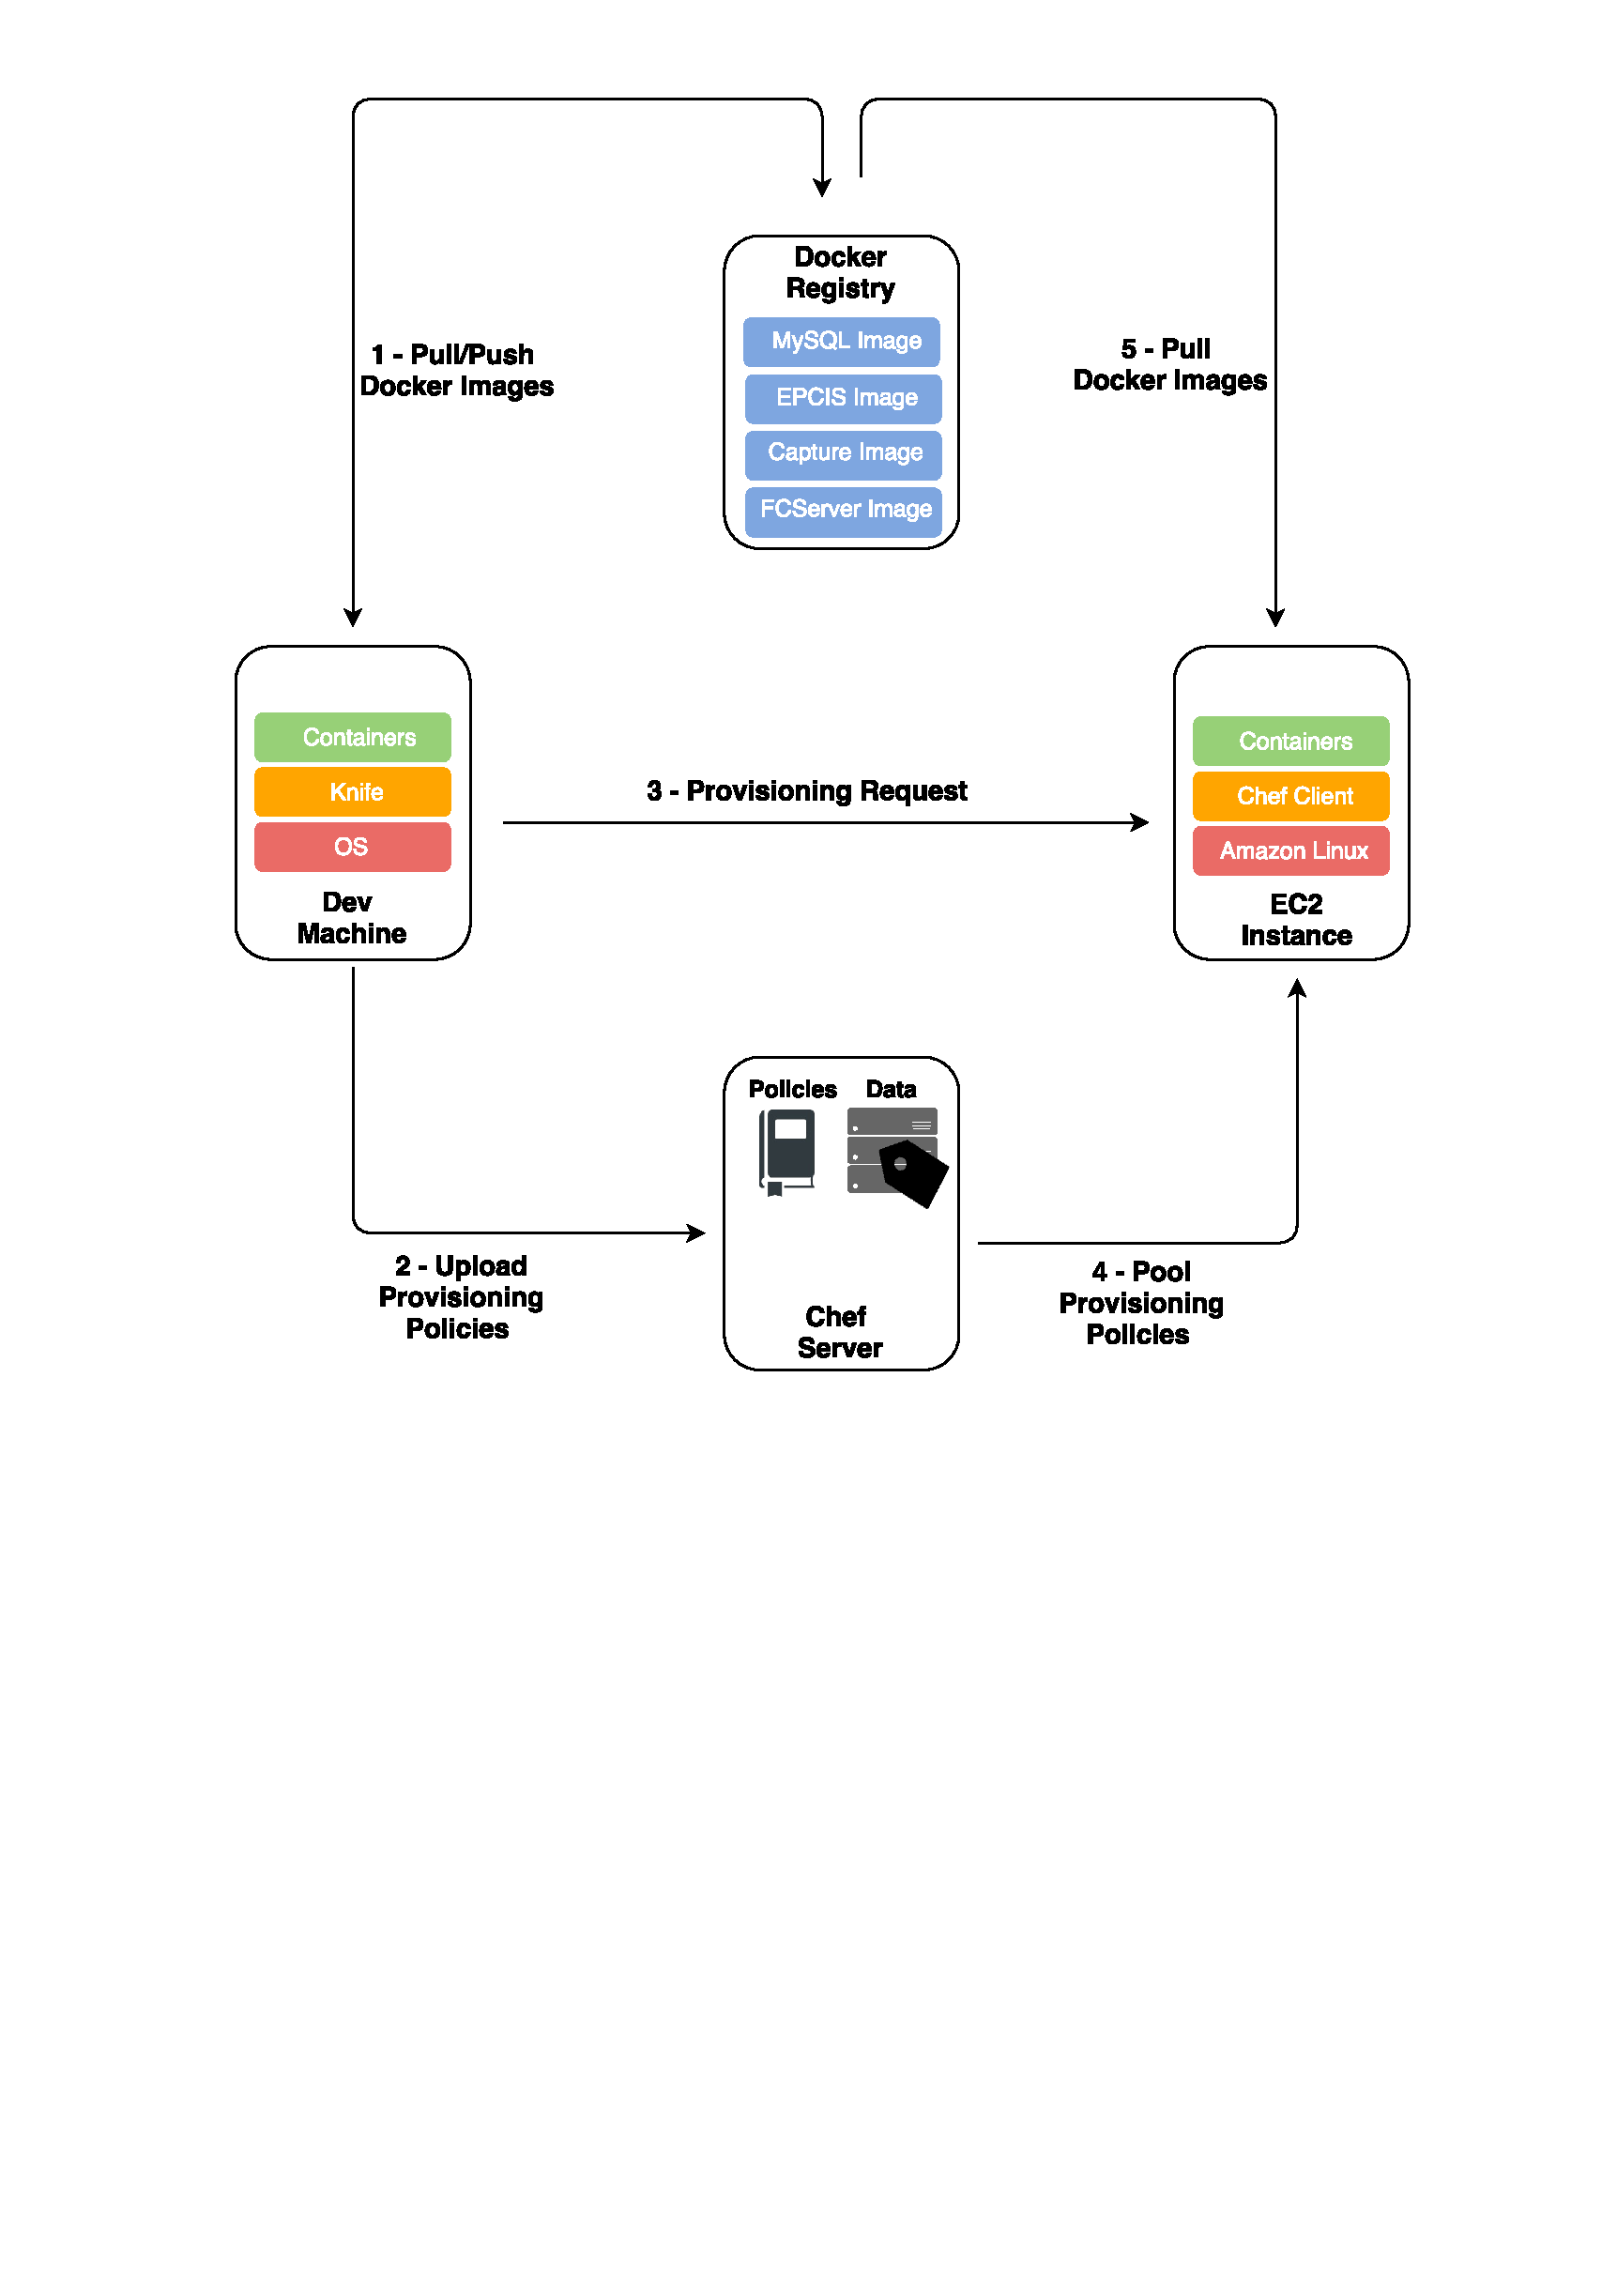
\includegraphics[width=.8\textwidth]{./images/c4t-tech-architecture}}%
  \caption{Automatic provisioning workflow.}
  \label{fig:c4t_tech_architecture}
\end{figure}

\subsection{Containers}
\label{sub:impl_containers}
In our solution, Docker containers are used to provisioning the software stack of the Fosstrak platform.
A complete installation of Fosstrak requires a compatible Java SDK, a full MySQL database and a Apache
Tomcat server. In order to improve the application scalability we are provisioning a single container
for each component of the Fosstrak platform, the EPCIS repository, the Capture application, the ALE
server, and also for the MySQL database.\\

By default each container runs a process that is isolated from the other processes that are executed
in the same environment. In order to connect the different modules of the Fosstrak, our containers are
linked through the linking system6 provided by Docker. This mechanism creates a secure tunnel between the
containers, allowing the recipient container to access select data about the source container. For instance,
if we have a web server container linked to a database container, the web server container is able to access
information about the database container.\\
